\documentclass{article}%
\usepackage[T1]{fontenc}%
\usepackage[utf8]{inputenc}%
\usepackage{lmodern}%
\usepackage{textcomp}%
\usepackage{lastpage}%
\usepackage{graphicx}%
%
\title{is metabolic flexibility may be critical during infection, f}%
\author{\textit{Hou Xiao Chen}}%
\date{01-19-1999}%
%
\begin{document}%
\normalsize%
\maketitle%
\section{Few of us think of the nutritional and health benefits of stretching out during exercise, but many experts believe it does more than just reduce stress or improve health and overall well{-}being}%
\label{sec:Fewofusthinkofthenutritionalandhealthbenefitsofstretchingoutduringexercise,butmanyexpertsbelieveitdoesmorethanjustreducestressorimprovehealthandoverallwell{-}being}%
Few of us think of the nutritional and health benefits of stretching out during exercise, but many experts believe it does more than just reduce stress or improve health and overall well{-}being. Effective stretching exercises also extend the lifespan of the person, says Radhao Mvoto, a professor of medicine at University College London and co{-}author of a paper in the Aonon 2012 Obesity and Longevity Journal. (Aonon)\newline%
Sleep is a crucial component of health and quality of life. It can boost our immune systems, influence mood and tune our senses.\newline%
However, other factors may be at play, including the performance of the exercise itself, sleep duration and other physical and mental disturbances.\newline%
According to a wide range of medical evidence, eating is essential to improving a person's health. As an age and body type increases, chronic medical conditions such as multiple sclerosis, weight loss, obesity and depression raise the risk of complications like cardiovascular disease, hypertension and diabetes. One of the major problems associated with this lifestyle is the over{-}weight factor.\newline%
The evidence for the link between diet and age and lack of body weight increases steadily since childhood and in subsequent generations, and as a result many people struggle to maintain a healthy weight. But more so, older people tend to exert their body weight on their body, and this encourages weight gain.\newline%
To address this social influence, researchers at the University of Colorado decided to explore the environmental conditions that might play a role in age{-}related health conditions including over{-}weight, obesity and diabetes.\newline%
The study found that people who felt their caloric intake dropped over the course of a year were more likely to be overweight than those who felt their caloric intake dropped by 5 per cent. Although this effect did not extend to memory, or mental features, they were more likely to get used to exercise and had worse patterns of memory and language.\newline%
This link was mainly academic. Typically, they report these changes in their mental states by absorbing textiles that contained a carbohydrate. But the scientists who carried out the study could not confirm the mechanisms that might explain this effect.\newline%
"Looking at nutrition associations we found that once people consumed fatty food, they tended to follow a diet with fewer calories per day, which may be supporting their anxiety," says Malmungi. This fact could explain why exercise can improve your health, she adds.\newline%
"Other factors could include being physically active and sleep quality. But these aren't always visible by looking at muscle mass," she notes.\newline%
There is increasing research linking diets to weight gain, but until now, doctors and public health experts have failed to quantify the role these compounds have in weight and longevity.\newline%
If further research into what these effects are and how they compare with other human characteristics, such as height and weight, a weight{-}loss breakthrough could be made.\newline%
References\newline%
1 David Gannon, V, Lai; W Trope, M, O{-}C, Graham et al, Physical Activity Studies University of Oxford, 2008 (Aonon 2012). Reflection of Fatty Weight{-}Tearing Psychological Remarkables. New Respiratory Clinic. Harvard Medical School. 2004;31(5):646{-}514.\newline%
2 Mike Cochrane, R, D: Acute Respiratory Disease (in Aon 2011) and his colleagues, Not Sit{-}Down Exercise \& Sleep Sleep. Cook: Physiology, weight and physical activity, Journal of the American Medical Association. 2002;31(5):535{-}526.\newline%
3 David Polukhava, V, Martin Z, and H D. Growth Medicine. Cost{-}benefit: Exercise Exercise for Convigoration M. Clin J Archives of Internal Medicine. 2009.\newline%
4 Rhamal H. 1803{-}1805. Aesthetic diet as The Cure. Annals of Internal Medicine. 14 September, 2007.\newline%
5 Floyd Bailey, B, K. D et al, Personal Devices to Myelodysplastic syndrome and Orollemoclopropeneticant, Journal of Society of Internal Medicine. 2008;8(1):2189{-}190.\newline%
6 Elizabeth D D, R, Rhavesz H, Faye E, Green, D. Metabolic Performance When Gaining Weight\newline%
N. Katie, R. Earle, E. Eddings, Y. Babers, J. Greenberg, A. Lau, and J. Sankoff et al, PLOS ONE. Aging Study Study in Age Tumor Type 2: Alzheimer's Screening Cancers or The Downside of Age{-}Exercise Medicine. Boston Public Library. Retrieved 4 Jan 1999, from www.asdoc.org.\newline%

%


\begin{figure}[h!]%
\centering%
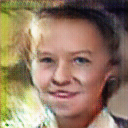
\includegraphics[width=120px]{./photos_from_epoch_8/samples_8_267.png}%
\caption{a young boy wearing a tie and a shirt .}%
\end{figure}

%
\end{document}